\chapter{引言}\label{cha:introduction}
\section{选题背景与意义}
\label{sec:background}
医学影像中的疾病标记物是一种生物特征,或可在图像中检测到的疾病标志物。医学影像中的视觉疾病标记物是专业医师评估特定疾病的风险,类别和状态的重要指标。专业医师在诊断过程中,必然会遇到难以诊断的病例。而疾病标记物作为一种可以做出可靠诊断的有效手段,其实用性已经在临床使用中被证明。

在医学影像中,疾病标志物是与患者诊断相关的图像特征。例如,许多疾病标记物经常用于确定肺癌的风险。通过X射线,电子计算机断层扫描仪(Computed Tomography,缩写为CT)或核磁共振成像(Magnetic Resonance Imaging,缩写为MRI)检测到的简单的肺部病变可诊断为疑似肿瘤。病变本身可作为疾病标记物,病变的微小细节也可作为疾病标记物,并可共同用于评估肿瘤的风险。如肺结节评估中使用的一些成像疾病标记物包括大小、针刺、钙化、空化、肺内位置、生长速率和代谢速率,这些疾病标记物可综合诊断肺癌,以给出合理科学的诊断结果。除此之外,还可以使用多种技术(例如肺部CT或者MRI、脑电图、脑磁图、皮肤镜图像及其各种医学影像设备)测量成像疾病标记物。为了让读者对医学图像中的疾病标记物有较为直观的认识,如图\ref{mul_fig:medical_imaging_biomarkers_examplar}所示,本文列出了四张包含疾病标记物的眼底图像,由于眼底图像中疾病标记物分布较为广泛(比如,图中第一列图像),我们只标出图像中具有典型特性的疾病标记物。
\begin{figure}[h]
	\centering
	\includegraphics[width=1.0\textwidth]{figure/typical_biomarkers_examplar}
	\caption[眼底图像中的疾病标记物示例]{眼底图像中的疾病标记物示例(图中红色箭头指示疾病标记物)。}
	\label{mul_fig:medical_imaging_biomarkers_examplar}
\end{figure}

疾病标记物在临床医学中可发挥重要作用,可用于处理疾病诊断、疾病风险预测、疾病类型区分等多个问题。而利用计算机技术在医学影像上实现对疾病标记物的自动定位,可为发现更多潜在疾病标记物提供技术支持,同时也能为影像科医师减轻一定工作量,有利于将影像科医师从繁重的工作中解放出来。
% overview of weakly supervised object localization:https://www.jianshu.com/p/e0097769f3b3
\section{研究内容与主要难点}\label{sec:existing_diffcuities}
\subsection{研究内容}
本文旨在在弱监督条件下,精确定位到医学图像中的疾病标记物。该任务会提供图像级标签(正常/异常),针对一张输入图像中有一个或者多个疾病标记物(疾病标记物数量不确定,可能有一个,也可能有多个,还可能没有即正常)的情况,该任务要求从像素层面上将疾病标记物和背景(正常区域)完全分离出来。更准确地说,该任务是为图像中的每个像素分配标签(正常/异常),以给出疾病标记物的像素级定位结果,其中具有相同标签的像素表示具有某些共同的特征。
\subsection{主要难点}
在弱监督条件下,实现疾病标记物的精确定位,临床意义重大,同时也存在诸多难点,是一个困难与挑战并存的任务。对于疾病标记物的粗略位置定位,目前已有很多相关工作可供参考,例如,多示例学习、卷积神经网络(Convolutional Neural Networks,缩写为CNN)的可视化和计算机视觉领域的弱监督目标定位。一旦要求疾病标记物的精确位置,直接相关工作寥寥无几,这本身就给这一问题增大了许多难度。另外,医学图像中疾病标记物往往分布广泛、并且具有不规则形状和大小,疾病标记物与背景正常区域相似度也极高(比如CT或者MRI图像、眼底图像)。对于图像中极其细微、难以察觉的疾病标记物,专业医师也容易混淆或者遗漏。另外,与各个物体边界都明确清晰、目标物体的形状数量也容易确定的自然图像相比,医学图像中疾病标记物与周围背景之间的边界要模糊得多,疾病标记物的数量也很难确定。对于发病率很低的某些特定疾病,比如,阿尔兹海默症,图像样本数量也远远没有自然图像丰富。这些都表明精确定位疾病标记物是一项极具挑战性的任务。以眼底图像中的疾病标记物举例而言,图\ref{fig:biomarker_localization_example}是一张包含了多种糖尿病性视网膜病变疾病标记物的眼底图像。图中红色矩形框、绿色矩形框、蓝色矩形框和黄色矩形框标记了四种糖尿病性视网膜病变的疾病标记物,分别代表软性渗出液(Soft Exudates)、微动脉瘤(Microaneurysms)、硬性渗出液(Hard Exudates)和出血(Hemorrhages)。可以发现,这张眼底图像具有复杂的纹理结构。从颜色特征上看,出血(黄色矩形框)与微动脉瘤(绿色矩形框)和眼底血管非常相似,而且极其细微,难以被察觉。从分布位置上看,图中各个位置(比如,图像左下角、中间和右上角)均包含疾病标记物。图中四种疾病标记的数量及其边界也无法确定。以上都说明弱监督条件下精确定位疾病标记物并不是一个容易的任务。
\begin{figure}[h!]
	\centering
	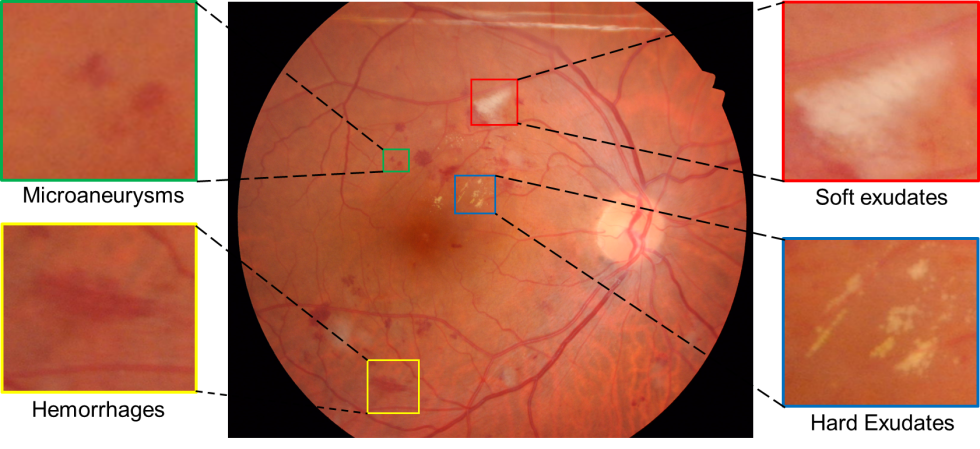
\includegraphics[width=1.0\textwidth]{figure/biomarker_localization_example}
	\caption[眼底图像中糖尿病性视网膜病变对应的多种疾病标记物示例]{眼底图像中糖尿病性视网膜病变对应的多种疾病标记物示例。} 
	\label{fig:biomarker_localization_example}
\end{figure}
\section{论文结构与章节安排}\label{sec:arrangement}
本文将会用六章的内容,仔细而全面的介绍本文提出的精确定位疾病标记物方法,并在相关数据集上完成实验验证,各章内容安排如下:
%https://stackoverflow.com/questions/2740437/changing-style-of-latex-description-lists
%https://latex.org/forum/viewtopic.php?t=7607
\begin{description}[style=multiline,leftmargin=1.7cm]
	\item[第一章:] 绪论。本章将叙述与疾病标记物定位任务相关的背景知识。此外,我们还将概述本文的研究内容及其主要难点。
	\item[第二章:] 相关研究基础。本章将介绍后文用到的相关技术和相关研究进展。随后此章还将介绍后文实验中所使用的评价标准和与疾病标记物定位相关的主流数据集。
	\item[第三章:] 疾病标记物的自动定位方法。本章将详细描述我们针对疾病标记物定位任务提出的解决方法。具体而言,本章将首先描述本文的研究问题和解决思路,据此我们给出本文提出的方法、模型结构、训练策略和损失函数。最后,本文将用一张算法流程图用形式化语言描述网络训练过程。
	\item[第四章:] 二类疾病标记物定位的实验评估。本章将利用本文提出的模型在两个二类数据集上进行相关实验。本文还将针对本文提出的模型本身,设计一系列消融实验。最后,本文设置多组不同的实验参数,以探讨本文提出的方法的鲁棒性。
	\item[第五章:] 多类疾病标记物定位的实验评估。与第四章类似,此章将利用本文提出的模型在一个多类数据集上进行相关实验。
	\item[第六章:] 总结与展望。此章将对全文工作进行总结性描述,并明确未来研究方向。
\end{description}